
\documentclass[journal,12pt,twocolumn]{article}
\usepackage{graphicx}
\usepackage[none]{hyphenat}
\usepackage[margin=0.5in]{geometry}
\usepackage[cmex10]{amsmath}
\usepackage{array}
\usepackage{booktabs}
\usepackage{gensymb}
\usepackage{textcomp}
\title{\textbf{Conic Assignment}}
\author{Manideep Parusha - FWC22004}
\date{\today}

\providecommand{\norm}[1]{\left\lVert#1\right\rVert}
\providecommand{\abs}[1]{\left\vert#1\right\vert}
\let\vec\mathbf
\newcommand{\myvec}[1]{\ensuremath{\begin{pmatrix}#1\end{pmatrix}}}
\newcommand{\mydet}[1]{\ensuremath{\begin{vmatrix}#1\end{vmatrix}}}
\providecommand{\brak}[1]{\ensuremath{\left(#1\right)}}
\let\vec\mathbf
\begin{document}

\maketitle
\section*{Problem}
\paragraph{A is a point on the parabola $y^2 = 4ax$. The normal at $\vec{A}$ cuts the parabola again at point $\vec{B}$. If $\vec{AB}$ subtends a right angle at the vertex of the parabola, find the slope of AB.}

\section*{Solution}

\begin{figure}[h!]
\centering
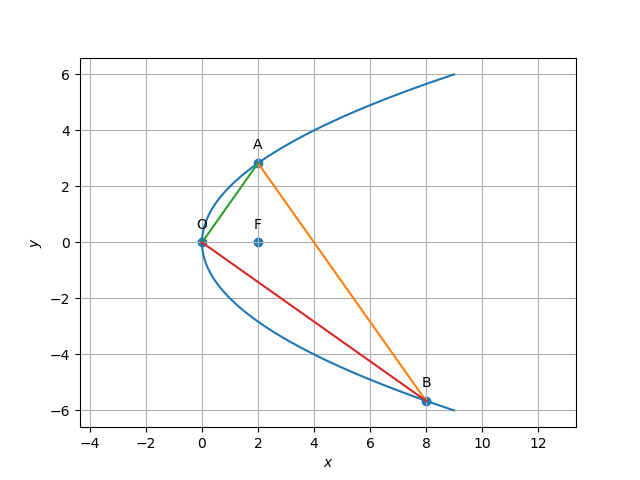
\includegraphics[width=\columnwidth]{figs/plot_con.png}
	\caption{parabola with normal at A}
\label{fig:con_py}
\end{figure}

\subsection*{Construction}
Input taken for the construction of the parabola are it's focus and directrtx.

\begin{table}[h]
	\centering
\setlength\extrarowheight{2pt}
	\begin{tabular}{|c|c|c|}
		\hline
		\textbf{Symbol} & \textbf{Value} & \textbf{Description} \\
		\hline
		O & \myvec{0\\0} & vertex\\
		\hline
		A & \myvec{a_1\\a_2} & point on parabola\\
		\hline
		B & \myvec{b_1\\b_2} & point on parabola\\
		\hline
		F & \myvec{2,0} & Focus of the parabola\\
		\hline
	\end{tabular}
\end{table}
From the given equation of the parabola, we can assume the points $\vec{A}\&\vec{B}$ as 
\begin{align}
	\vec{A} = \myvec{a_1\\a_2} = \myvec{2\\2\sqrt{2}}
\end{align}
%Radius of the circle is the distance between center and any point on circle.
%\begin{align}
%	r = \norm{A-C}\\
%	r = \sqrt{13}
%\end{align}

The given equation of the parabola is $y^2 = 4ax$, which can be expressed also as
\begin{equation}
	\vec{x}^T\vec{V}\vec{x} + 2\vec{u}^T\vec{x} = 0
	\label{par}
\end{equation}
where
\begin{align}
	\vec{V} = \myvec{0&0\\0&1} \\
	\vec{u}= \myvec{-2 \\ 0} \\
	f = 0
\end{align}
We know that the point $\vec{A}$ lies on the parabola and 
the normal at $\vec{A}$ can be calculated as
\begin{align}
	\vec{n} = \vec{V}\vec{A} + \vec{u}	
	\label{eq:normal}
\end{align}
Given that the normal passes through $\vec{A} \& \vec{B}$
\begin{align}
	L : \vec{x} = \vec{A} + \mu_i \vec{n}  
\end{align}
intersection with conic in eqn \eqref{par}
\begin{align}
	\mu_1 = 0\\
	\mu_2 = -3
\end{align}
the point $\vec{B}$  
\begin{align}
	\vec{B} = \vec{A} + \mu_2\vec{n}
\end{align}
The slope of $\vec{AB}$ can be calculated as
\begin{align}
	\vec{B-A} = \myvec{6\\-6\sqrt{2}}\\
	\implies \vec{m} = \myvec{1\\m}\\
	\implies m = -\sqrt{2}
\end{align}
	Hence,  the slope of the normal $\vec{AB}$ is $-\sqrt{2}$.
\end{document}
